\chapter{Landasan Teori}
\label{chap:definition}

\section{\textsl{Data Mining}}

\textsl{Data mining} merupakan merupakan proses yang melakukan pengambilan inti sari atau penggalian \textsl{knowledge} dari data yang besar dan merupakan salah satu langkah dari \textsl{knowledge discovery}.

Menurut [1], \textsl{knowledge discovery} dapat dibagi menjadi 7 tahap (gambar 2.1):
\begin{enumerate}
	\item \textsl{Data cleaning}
	\item \textsl{Data integration}
	\item \textsl{Data selection}
	\item \textsl{Data transformation}
	\item \textsl {Data mining}
	\item \textsl{Pattern Evaluation}
	\item \textsl{Knowledge presentation}
\end{enumerate}

\begin{figure}
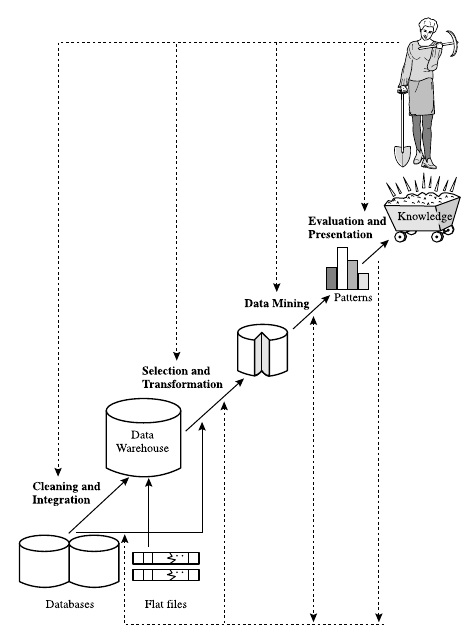
\includegraphics[scale=1]{Gambar/tahapdatamining.jpg}
\caption[Tahap \textsl{Data Mining}, Sumber Data Mining Concepts and Techniques]{Tahap \textsl{Data Mining}, Sumber Data Mining Concepts and Techniques} 
\end{figure}

Tahap pertama hingga keempat merupakan bagian dari \textsl{data preprocessing}, dimana data-data disiapkan untuk dilakukan penggalian data. Tahap \textsl{data mining} merupakan tahap dimana melakukan penggalian data. Tahap keenam merupakan tahap pencarian pola yang merepresentasikan \textsl{knowledge}. Sedangkan tahap terakhir merupakan visualisasi dan representasi dari \textsl{knowledge} yang sudah diperoleh dari tahap sebelumnya.


\subsection{\textsl{Data Cleaning}}
\textsl{Data cleaning} merupakan tahap \textsl{data mining} untuk menghilangkan \textsl{missing value} dan \textsl{noisy data}. Pada umumnya, \textsl{data} yang diperoleh dari \textsl{database} terdapat nilai yang tidak sempurna seperti nilai yang hilang, nilai yang tidak valid atau bahkan salah ketik. Nilai-nilai tersebut dapat diatasi dengan cara \textsl{smoothing techniques}. Atribut dari suatu \textsl{database} yang tidak relevan atau redudansi bisa diatasi dengan menghapus atribut tersebut. 

\subsubsection{\textsl{Missing Values}}
\textsl{Missing values} akan mengganggu proses \textsl{data mining} pada komputer dan dapat menghasilkan nilai akhir yang tidak sesuai. Terdapat beberapa teknik untuk mengatasi \textsl{missing values} yaitu
	\begin{itemize}
		\item Membuang tuple yang terdapat nilai yang hilang\textit{\textit{}}
		\item Mengisi nilai yang hilang secara manual
		\item Mengisi nilai yang hilang dengan menggunakan nilai konstan yang bersifat umum
		\item Menggunakan nilai rata-rata dari suatu atribut untuk mengisi nilai yang hilang
	\end{itemize}
\subsubsection{\textsl{Noisy Data}}
\textsl{Noisy data} merupakan nilai yang berasal dari error atau tidak valid. \textsl{Noisy data} dapat dihilangkan dengan menggunakan teknik \textsl{smoothing}. Terdapat 3 metode untuk menghilangkan \textsl{noisy data} yaitu
	\begin{itemize}
		\item \textsl{Binning}, merupakan metode pengisian data sesuai dengan proses yang dilakukan pada data tersebut
		\item \textsl{Regression}, merupakan metode yang mencari persamaan atribut untuk memprediksikan suatu nilai
		\item	\textsl{Clustering}, merupakan metode pengelompokan dimana ditemukan \textsl{outliers} yang dapat dibuang
	\end{itemize}

%\subsubsection{\textsl{Data Cleaning as a Process}}
%Tahap pertama pada \textsl{data cleaning} adalah \textsl{discrepancy detection}. Ketidakcocokan dapat dikarenakan oleh beberapa faktor, termasuk desain data yang buruk, kesalahan manusia ketika memasukan data, dan data yang sudah kadarluarsa. Ketidakcocokan ini juga dapat disebabkan tidak konsisten representasi data dan kode atau dikarenakan kesalahan perangkat ketika melakukan pemasukan data.

%Untuk mempermudah pencarian ketidakcocokan tersebut, kita dapat membuat sebuah data yang berisi informasi mengenai data atau biasa disebut \textsl{metadata}. Pada tahap ini, penulisan \textsl{script} bisa ditulis dengan cara masing-masing. Disini, dapat ditemukan \textsl{noise}, \textsl{outliers}, dan nilai-nilai yang tidak cocok atau tidak konsisten.

%Data juga harus diperiksa dengan \textsl{unique rules}, \textsl{consecutive rules}, dan \textsl{null rules}. \textsl{unique rules} mengatakan bahwa setiap nilai dari sebuah atribut harus berbeda dengan nilai yang lain pada atribut tersebut. \textsl{Consecutive rules} mengatakan bahwa tidak boleh ada nilai yang hilang diantara nilai tertinggi dan terendah untuk sebuah atribut, dan semua nilai harus bersifat unik. \textsl{null rules} menspesifikasikan penggunaan nilai \textsl{blanks} atau kosong, tanda tanya, karakter spesial, atau \textsl{string} yang dapat menandakan bahwa nilai tersebut bersifat kosong.

%Tahap deteksi ketidakcocokan ini dapat dibantu juga dengan menggunakan \textbf{data scrubbing tools} dan \textbf{data auditing tools}. \textbf{data scrubbing tools} akan menggunakan sebuah domain data untuk melakukan pencarian ketidakcocokan data dan membetulkan data tersebut dengan menggunakan teknik \textsl{parsing} dan \textsl{fuzzy matching}. \textbf{Data auditing tools} akan mencari ketidakcocokan dengan melakukan analisa data untuk menemukan \textsl{rules}, relasi, dan mendeteksi data yang melanggar hal tersebut.

%Beberapa data dapat diperbaiki dengan cara manual, namun sebagian besar data akan membutuhkan \textsl{data transformation} untuk membetulkan data tersebut.

\subsection{\textsl{Data Integration}}
\textsl{Data integration} merupakan tahap menggabungkan data dari berbagai sumber. Sumber tersebut bisa termasuk beberapa \textsl{database}, \textsl{data cubes}, atau bahkan \textsl{flat data}. Tahap ini harus dilakukan secara teliti terutama ketika dalam memasangkan nilai-nilai yang berasal dari sumber yang berbeda. Pada tahap ini, perlu dilakukan identifikasi data apakah data tersebut dapat diturunkan atau tidak agar data yang diperoleh tidak terlalu besar.
\textsl{Data integration} yang baik merupakan integrasi yang dapat memaksimalkan kecepatan dan meningkatkan akurasi dari proses \textsl{data mining}. 

\subsection{\textsl{Data Selection}}
Proses dimana data-data yang relevan dengan analisis akan diambil dari database dan data yang tidak relevan akan dibuang. Sebagai contoh kasus, jika akan dilakukan analisa mengenai nilai mahasiswa dalam satu semester, atribut pada tabel nilai sebagai berikut
	\begin{itemize}
		\item NPMMahasiswa
		\item NamaMahasiswa
		\item JenisKelamin
		\item Alamat
		\item MataKuliah
		\item NilaiART
		\item NilaiUTS
		\item NilaiUAS
	\end{itemize}
Maka, atribut yang akan diambil adalah MataKuliah, NilaiART, NilaiUTS, NilaiUAS, sedangkan atribut yang akan dibuang adalah NPMMahasiswa, NamaMahasiswa JenisKelamin, dan Alamat karena tidak terlalu berhubungan dengan analisa.

\subsection{\textsl{Data Transformation}}
\textsl{Data transformation} merupakan tahap pengubahan data agar siap dilakukan proses \textsl{data mining}. \textsl{Data transformation} bisa melibatkan,
	\begin{itemize}
		\item \textsl{Smoothing}, proses untuk membuang \textsl{noise} seperti yang dilakukan pada tahap \textsl{data cleaning}
		\item \textsl{Aggregation}, proses mengganti nilai-nilai menjadi suatu nilai yang dapat mewakili nilai sebelumnya
		\item \textsl{Generalization}, proses dimana membuat suatu nilai yang bersifat khusus menjadi nilai yang bersifat umum
		\item \textsl{Normalization}, proses dimana suatu nilai dapat diubah skalanya menjadi nilai yang lebih kecil dan spesifik
		\item \textsl{Attribute construction}, proses membuat atribut baru yang berasal dari beberapa atribut untuk membantu proses data mining
	\end{itemize}
--tanyakan!!!-->Proses \textsl{smoothing} merupakan proses yang sama seperti pada tahap \textsl{data cleaning}.<---tanyakan!!!--

\subsubsection{\textsl{Normalization}}
Atribut dapat dinormalisasi dengan memberi skala pada nilainya sehingga nilai tersebut menjadi suatu range yang lebih spesifik dan kecil seperti 0,0 sampai 1,0.
Dua teknik nnormalisasi yaitu, \textsl{min-max normalization} dan \textsl{z-score normalization}. \textsl{Min-max normalization} akan mengubah semua nilai menjadi nilai dengan skala tertentu. Dengan menggunakan rumus 

\begin{displaymath}
	\nu' = \frac{\nu-min_{A}}{max_{A}-min_{A}}(newMax_{A}-newMin_{A})+newMin_{A}	
\end{displaymath}

Contoh kasus, misalkan nilai minimun dan maximum dari suatu pendapatan adalah 12.000 dan 98.000, akan diubah menjadi berskala antara 0,0 sampai 1,0. Jika ada nilai pendapat yang baru, yaitu 73.600, maka akan menjadi

\begin{displaymath}
\frac{73.600-12.000}{98.000-12.000} (1,0-0)+0 = 0,716
\end{displaymath}

\textsl{z-score normalization} merupakan normalisasi berdasarkan nilai rata-rata dan standar deviasi dari nilai-nilai atribut dengan cara

\begin{displaymath}
\nu' = \frac{\nu-\overline{A}}{\sigma_{A}}
\end{displaymath}

Contoh kasus, misal nilai rata-rata dan standar deviasi dari nilai-nilai atribut pendapatan adalah 54.000 dan 16.000. Dengan \textsl{z-score}, jika ada nilai pendapatan baru yaitu 73600, maka akan diubah menjadi

\begin{displaymath}
\frac{73.600-54.000}{16.000} = 1,225 
\end{displaymath}

\subsubsection{\textsl{Attribute Construction}}
\textsl{Attribute Construction} merupakan teknik menambahkan atribut baru yang berdasarkan dari atribut yang sudah ada guna menambah akurasi. Contoh kasus, dibuat atribut baru bernama area berdasarkan atribut panjang dan lebar. 

\subsubsection{\textsl{Data Reduction}}
Proses \textsl{aggregation} dan \textsl{generalization} akan dilakukan dalam bentuk proses \textsl{data reduction} dan \textsl{Data Cube Aggregation}.
\textsl{Data reduction} dan dilakukan untuk mendapatkan nilai yang representif namun tetap menjaga keakuratan hasil \textsl{data mining}. Terdapat beberapa cara dalam mengimplementasikan \textsl{data reduction} yaitu
	\begin{itemize}
		\item \textsl{Data subset selection}
		\item \textsl{Dimensionality reduction}
		\item \textsl{Numerosity reduction}
		\item \textsl{Discretization and concept hierarchy generation}
	\end{itemize}	

\subsubsection {\textsl{Attribute Subset Selection}}
\textsl{Attribute subset selection} merupakan salah satu cara melakukan \textsl{data reduction} dengan menghilangkan atribut-atribut yang tidak relevan atau data yang redudansi. Hal ini dapat mempermudah pencarian pola dikarenakan banyak atribut yang muncul akan berkurangnya. 

\subsubsection {\textsl{Dimensionality Reduction}}
\textsl{Dimensionality Reduction} merupakan metode pengurangan nilai secara acak dengan cara melakukan konversi data. Jika data original dapat dibuat ulang dari data yang sudah dikompresi tanpa kehilangan informasi, maka akan dikatakan \textsl{lossless}, namun jika hanya mendapatkan data pendekatannya saja, akan disebut lossly [1].

\subsubsection {\textsl{Numerosity Reduction}}
\textsl{Numerosity Reduction} merupakan metode dimana data diganti atau ditentukan dengan cara parametik atau nonparametrik.

\subsubsection {\textsl{Discretization and Concept Hierarchy Generation}}
lewat dulu

\subsection{\textsl{Data Mining}}

\subsubsection{\textsl{Classification and Prediction}}
\textsl{Classification} merupakan pemodelan yang dibangun untuk memprediksikan label kategori, seperti "`baik"', "`cukup"', dan "`buruk"' dalam sistem penilaian sikap seorang siswa atau "`mini bus"', "`bus"', atau "`sedan"' dalam kategori tipe mobil. Kategori tersebut dapat direpresentasikan dengan menggunakan nilai \textsl{discrete}. Nilai \textsl{discrete} merupakan nilai yang terpisah dan berbeda, seperti 1 atau 5. Kategori yang direpresentasikan oleh nilai \textsl{discrete} maka akan menjadi nilai yang terurut dan tidak memiliki arti, seperti 1,2,3 untuk merepresentasikan kategori tipe mobil "`mini bus"', "`bus"', dan "`sedan"'.

\textsl{Prediction} merupakan model yang dibangun untuk meramalkan \textsl{continuous-value function} atau \textsl{ordered value}. \textsl{Ordered value} merupakan nilai yang terurut dan berlanjut. contoh studi kasus untuk pemodelan prediction adalah seorang marketing ingin meramalkan seberapa banyak konsumen yang akan belanja di sebuah toko dalam waktu satu bulan. Pemodelan tersebut disebut \textsl{predictor}.\textsl{Regression Analysis}, merupakan metodologi statistik yang digunakan untuk \textsl{numeric prediction}. \textsl{Classification} dan \textsl{numeric prediction} merupakan dua jenis utama dalam masalah prediksi.

\textsl{Data Classification} merupakan proses untuk melakukan klasifikasi. \textsl{Data classification} memiliki dua tahap proses, yaitu \textsl{learning step} dan tahap klasifikasi seperti pada ilustrasi di gambar 2.2. \textsl{Learning step} merupakan langkah pembelajaran, di mana algoritma klasifikasi membangun \textsl{classification rules} (yang berisi syarat atau aturan sebuah nilai masuk ke dalam kategori tertentu) dengan cara menganalisis \textsl{training set} yang merupakan \textsl{database tuple}. Karena pembuatan \textsl{classification rules} menggunakan \textsl{training set}, yang dikenal juga sebagai \textsl{supervised learning}. 
Pada tahap kedua, dilakukan proses klasifikasi nilai berdasarkan \textsl{classification rules} yang sudah dibangun dari tahap pertama.

\begin{figure}
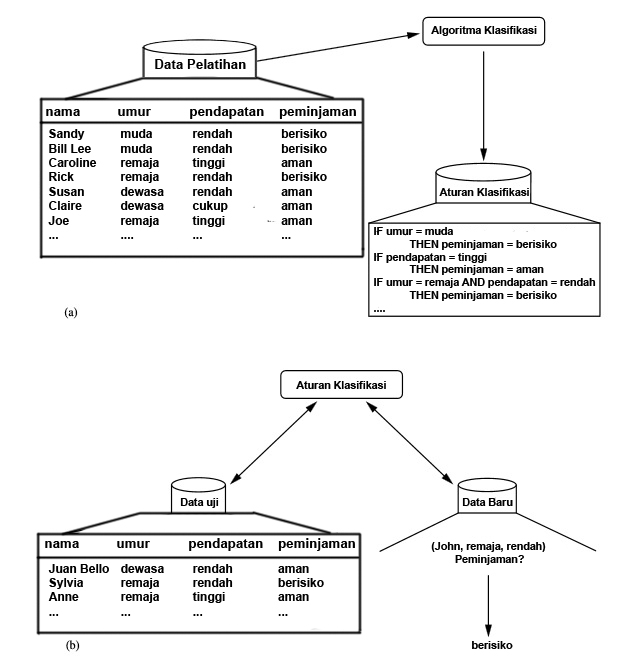
\includegraphics[scale=1]{Gambar/tahapdataclassification.jpg}
\caption[Tahap \textsl{Data Mining}, Sumber Data Mining Concepts and Techniques]{proses \textsl{data classification}, Sumber Data Mining Concepts and Techniques} 
\end{figure}

\subsection{\textsl{Decision Tree}}
Salah satu cara pembuatan \textsl{classification rules} pada \textsl{Data Classification} adalah dengan membuat \textsl{decision tree} (pohon keputusan). \textsl{Decision tree} merupakan \textsl{flowchart} yang berbentuk pohon, dimana setiap node internal (\textsl{nonleaf} node) merupakan hasil test dari atribut, setiap cabang merepresentasikan output dari test, dan setiap node daun memiliki \textsl{class label}. Bagian paling atas dari pohon disebut \textsl{root node}. Contoh studi kasus, pohon keputusan untuk menentukan apakah seorang konsumen akan membeli komputer atau tidak (ilustrasi pohon keputusan pada gambar 2.3) 

\begin{figure}
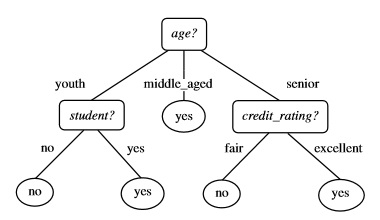
\includegraphics[scale=1]{Gambar/decisiontree.jpg}
\caption[Tahap \textsl{Data Mining}, Sumber Data Mining Concepts and Techniques]{proses \textsl{data classification}, Sumber Data Mining Concepts and Techniques} 
\end{figure}

subsubsection{\textsl{Decision Tree Induction}}
\textsl{Decision tree induction} merupakan pelatihan pohon keputusan dari tupel pelatihan kelas berlabel. Terdapat tiga teknik untuk membuat \textsl{decission tree} yaitu ID3, C4.5 dan Classification and Regression Trees (CART). ketiga teknik tersebut menggunakan pendekatan \textsl{greedy} yang merupakan \textsl{decission tree} yang dibangun secara \textsl{top-down recursive divide and conquer}. Berikut algoritma untuk membuat pohon keputusan dari suatu tupel pelatihan.

Input:
\begin{itemize}
	\item Partisi data, D, merupakan set data pelatihan dan kelas label
	\item \textsl{attribute\_list}, merupakan set dari atribut kandidat
	\item \textsl{Attribute\_selection\_method}, prosedur untuk menentukan \textsl{splitting criterion}. Pada input ini, terdapat juga data \textsl{splitting\_attribute} dan mungkin salah satu dari \textsl{split point} atau \textsl{splitting subset}
\end{itemize}

Output: pohon keputusan

Method:

(1) create a node N;

(2) if tuples in D are all of the same class, C then

(3)	return N as a leaf node labeled with the class C;

(4)	if attribute\_list is empty then

(5) return N as leaf node labeled with the majority class in D; //majority voting

(6)	apply Attribute\_selection\_method(D, atribute\_list) to find the "`best"' splitting\_criterion;

(7) label node N with splitting\_criterion;

(8) if splitting\_attribute is discrete valued and
				multiway splits allowed then //not restricted to binary trees
				attribute\_

(9) attribute\_list <- attribute\_list - splitting\_attribute; //remove splitting\_attribute

(10)for each outcome j of splitting\_criterion // partition the tuples and from subtrees for each partition

(11)let D\lowercase{j} be the set of data tuples in D satisfying outcome j; //a partition

(12) if D\lowercase{j} is empty then

(13) attach a leaf labeled with the majority class in D to node N;

(14) else attach the node returned by generate\_decision\_tree(D\lowercase{j}, attribute\_list) to node N;

endfor

(15) return N;

\subsection{\textsl{Pattern Evaluation}}
\textsl{Pattern evaluation} merupakan tahap mengidentifikasi apakah \textsl{pattern} atau pola tersebut menarik dan merepresentasikan \textsl{knowledge} berdasarkan beberapa \textsl{interestingness measures}.
Suatu \textsl{pattern} atau pola dapat dinyatakan menarik apabila
\begin{itemize}
	\item mudah dimengerti oleh manusia
	\item valid untuk data percobaan maupun data yang baru
	\item memiliki potensi atau berguna
	\item merepresentasikan \textsl{knowledge}
\end{itemize}

\subsection{\textsl{Knowledge Presentation}}
\textsl{Knowledge presentation} merupakan tahap representasi dan visualisasi terhadap \textsl{knowledge} yang merupakan hasil dari \textsl{knowledge discovery}.	
%\section{\textsl{Spatial and Spatiotemporal}}

\section{Log Histori KIRI}

KIRI memiliki log histori yang melakukan pencatatan untuk setiap user ketika menggunakan KIRI. \textsl{Log} tersebut memiliki 5 \textsl{field} untuk setiap \textsl{entry} sebagai berikut:
\begin{itemize}
	\item logId, primary key dari entry
	\item APIKey, mengidentifikasikan sumber dari pencarian ini
	\item \textsl{Timestamp} (UTC), waktu ketika pengguna KIRI mencari rute angkot menggunakan waktu UTC / GMT
	\item \textsl{Action}, tipe log, untuk penelitian ini selalu berisi FINDROUTE
	\item AdditionalData, mencatat koordinat awal, koordinat akhir, dan banyak rute yang ditemukan pada pencarian ini
\end{itemize}

LogId merupakan \textsl{field} dengan tipe data int dengan batas 6 karakter yang digunakan sebagai \textsl{primary key} dari tabel tersebut. LogId diisi dengan menggunakan fungsi \textsl{increment integer}. \textsl{Increment integer} merupakan fungsi untuk pengisian data pada database dengan menambahkan nilai 1 dari nilai yang terakhir kali diisi.
APIKey merupakan \textsl{field} dengan tipe data varchar yang digunakan untuk memeriksa pengguna KIRI ketika menggunakan KIRI.
\textsl{Timestamp} (UTC) merupakan \textsl{field} dengan tipe data \textsl{timestamp} yang digunakan untuk mencatat waktu penggunaan KIRI oleh user, diisi dengan menggunakan fungsi \textsl{current time}. \textsl{Current time} merupakan fungsi untuk pengisian data pada database dengan mengambil waktu pada komputer ketika record dibuat.
\textsl{Action} merupakan \textsl{field} dengan tipe data varchar yang digunakan untuk memeriksa fungsi apa yang dipanggil dari API KIRI. Terdapat beberapa tipe pada \textsl{field} ini, yaitu
/\begin{itemize}
	\item \textsl{ADDAPIKEY}, \textsl{action} yang dicatat ke dalam log ketika fungsi pembuatan \textsl{API key} yang baru dipanggil.
	\item \textsl{FINDROUTE}, \textsl{action} yang dicatat ketika user melakukan pencarian rute
	\item \textsl{LOGIN}, \textsl{action} yang dicatat ketika developers melakukan login dengan menggunakan \textsl{API key}
	\item \textsl{NEARBYTRANSPORT}, \textsl{action} yang dicatat ketika user mencari transportasi di daerah rute sedang dicari
	\item \textsl{PAGELOAD}, \textsl{action} yang dicatat ketika user memasuki halaman KIRI
 	\item \textsl{REGISTER},\textsl{action} yang dicatat ketika developers melakukan pendaftaran pada KIRI \textsl{API key}
	\item \textsl{SEARCHPLACE}, \textsl{action} yang dicatat ketika user memanggil fungsi pencarian lokasi dengan menggunakan nama tempat
	\item \textsl{WIDGETERROR}, mencatat log tersebut ketika user menerima error dari \textit{widget}
	\item \textsl{WIDGETLOAD}, mencatat log tersebut ketika user mengdownload widget
\end{itemize}
AdditionalData, merupakan \textsl{field} dengan tipe data varchar yang digunakan untuk mencatat informasi yang dibutuhkan sesuai dengan \textsl{field action}.